% Intended LaTeX compiler: xelatex
\documentclass[10pt, svgnames]{beamer}
\usepackage{graphicx}
\usepackage{longtable}
\usepackage{wrapfig}
\usepackage{rotating}
\usepackage[normalem]{ulem}
\usepackage{amsmath}
\usepackage{amssymb}
\usepackage{capt-of}
\usepackage{hyperref}
\usetheme{metropolis}
\author{Sappinandana Akamphon}
\date{}
\title{Power Transmission System Design}
\institute{ME TSE}
\usetikzlibrary{shapes,shapes.geometric}
\hypersetup{
 pdfauthor={Sappinandana Akamphon},
 pdftitle={Power Transmission System Design},
 pdfkeywords={},
 pdfsubject={},
 pdfcreator={Emacs 29.0.50 (Org mode 9.6)}, 
 pdflang={English}}
\begin{document}

\maketitle

\begin{frame}[label={sec:orgfa8502d}]{What We have Covered So Far}
\begin{itemize}
\item Shafts
\item Gears
\item Bearings
\item Flexible Elements
\item Power screws
\end{itemize}
\end{frame}

\begin{frame}[label={sec:org1dbb49b}]{Final Goal}
\begin{itemize}
\item Design a power transmission system \ldots{}

\item with multiple components \ldots{}

\item that interacts with one another \ldots{}
\end{itemize}
\end{frame}

\begin{frame}[label={sec:orgb07bb9c}]{Where Do We Start?}
\begin{itemize}
\item Given all the requirements: power, reduction ratio, speed ..
\item Which component should be designed first?
\end{itemize}
\end{frame}

\begin{frame}[label={sec:orgf953baf}]{System design is typically iterative}
\begin{itemize}
\item Possibly multiple correct solutions
\item Start from input or output
\item Proceed to the rest of the system
\item When contradiction arises, correct it
\item And redesign other parts to fix that mistake
\item Lather, rinse, repeat \ldots{}
\end{itemize}
\end{frame}

\begin{frame}[label={sec:orga6096b6}]{Order of Component Design}
\begin{enumerate}
\item Determine the required \(T\), \(v\), \(\omega\), \(H\), \ldots{}
\item Input - Output \(\rightarrow\) gear / chain + sprocket / pulley + belt / power screw
\item Determine forces on shaft
\item Shafts \(\rightarrow\) what the input and output are mounted on
\item Determine forces on bearings
\item Bearings \(\rightarrow\) what the shaft made contact with
\item Determine forces on joints
\item Joints: springs, bolts, welds, \ldots{}
\end{enumerate}

2, 4, 6, 8 \(\rightarrow\) already knows \\\empty
1, 3, 5, 7 \(\rightarrow\) need a little dust off
\end{frame}

\begin{frame}[label={sec:org2e83306}]{Determine Required T, V, \(\omega\), H}
\begin{itemize}
\item Problem usually gives a subset of mass, weight, torque, velocity, acceleration or \ldots{}

\item Need to determine \(F\) and \(T\) on shaft depending on mechanism involved
\end{itemize}
\end{frame}

\begin{frame}[label={sec:org19bbacf}]{Forces on Shaft}
\begin{center}
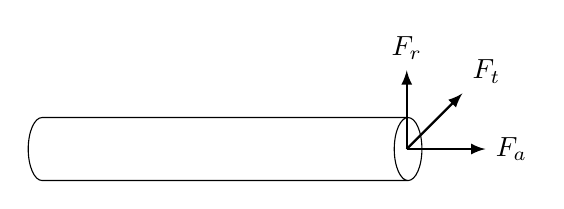
\begin{tikzpicture}[>=latex]
  \node[draw, cylinder, minimum height=5cm, minimum width=8mm, inner sep=5](shaft){};
  \draw [thick, ->] (shaft.east) ++ (180:0.2) node(O){} --++ (45:1) node[above right]{$F_{t}$};
  \draw [thick, ->] (O.center) --++ (90:1) node[above]{$F_{r}$};
  \draw [thick, ->] (O.center) --++ (0:1) node[right]{$F_{a}$};
\end{tikzpicture}
\end{center}
\normalcolor

2 directions possible:

\begin{itemize}
\item Radial Loads: any forces \(\perp\) shaft axis (\(F_{r}, F_{t}\))

\item Axial Loads: any forces \(\parallel\) shaft axis
\end{itemize}
\end{frame}

\begin{frame}[label={sec:org50585c4}]{Determine forces on shaft}
\begin{columns}
\begin{column}{0.5\columnwidth}
\begin{center}
\includegraphics[width=\textwidth]{./pictures/helical-gear-forces.png}
\end{center}
\end{column}

\begin{column}{0.5\columnwidth}
Gears: \(F_{a}, F_{t}, F_{r}\)

Forces on shaft:

\begin{itemize}
\item \(F_{a} \rightarrow\) Axial load on shaft
\item \(F_{r}\) and \(F_{t}\) \(\perp\) shaft axis \(\rightarrow\) Radial load on shaft = \(\sqrt{F_r^{2} + F_t^{2}}\)
\end{itemize}
\end{column}
\end{columns}
\end{frame}

\begin{frame}[label={sec:org543d0f2}]{Determining forces on shaft}
\begin{columns}
\begin{column}{0.6\columnwidth}
\begin{center}
\includegraphics[width=.9\linewidth]{./pictures/forces-on-pulley.png}
\end{center}
\end{column}

\begin{column}{0.5\columnwidth}
Pulleys + Belts: \(F_{1}, F_{2}\)

On shaft:

\begin{itemize}
\item \(F_{1}, F_{2}\) \(\perp\) shaft axis \(\rightarrow\) Radial load on shaft \(\approx\) \(F_{1} + F_{2}\)
\end{itemize}
\end{column}
\end{columns}
\end{frame}

\begin{frame}[label={sec:org84e7535}]{Determining forces on shaft}
\begin{columns}
\begin{column}{0.5\columnwidth}
\begin{center}
\includegraphics[width=.9\linewidth]{./pictures/chordal-speed-variation.png}
\end{center}
\end{column}

\begin{column}{0.5\columnwidth}
Chain + Sprocket: \(F_{1}\)

On shaft:

\begin{itemize}
\item \(F_{1}\) \(\perp\) shaft axis \(\rightarrow\) Radial load on shaft
\end{itemize}
\end{column}
\end{columns}
\end{frame}

\begin{frame}[label={sec:orgac13e38}]{Shaft Design}
\begin{itemize}
\item Radial load \(\rightarrow\) \(F_{r}\) \(\rightarrow\) bending stress
\item Axial load \(\rightarrow\) \(F_{a}\) \(\rightarrow\) axial stress
\item Torque \(\rightarrow\) \(T\) \(\rightarrow\) torsion
\end{itemize}

\begin{align*}
  \frac{1}{N_{s}} &= \frac{\sigma_{ae}}{S_{e}} + \frac{\sigma_{me}}{S_{y}} \\
  \sigma_{ae} &= \left( \sigma_{a}^{2} + 3 \tau_{a}^{2} \right)^{1/2} \\
  \sigma_{me} &= \left( \sigma_{m}^{2} + 3 \tau_{m}^{2} \right)^{1/2}
\end{align*}
\end{frame}

\begin{frame}[label={sec:orgc91ce0e}]{Bearing Design}
\begin{itemize}
\item Bearing equation needs radial load \(F_{r}\) and axial load \(F_{a}\)

\item Determine forces on bearings using equilibrium equations

\item Proceed to design bearings using \(F_{e}\) derived from \(F_{r}\) and \(F_{a}\)

\begin{align*}
  L &= L_R K_r \left( \frac{C}{F_e} \right)^{10/3} \\
  C &= F_e \left( \frac{L}{K_r L_R} \right)^{0.3}
\end{align*}
\end{itemize}
\end{frame}

\begin{frame}[label={sec:orgf6551e6}]{Forces on Joints}
\begin{itemize}
\item Consider forces of components attached to joints

\item Use equilibrium equation to determine the forces
\end{itemize}
\end{frame}

\begin{frame}[label={sec:orgf0feb29}]{Example}
A motor drive is used to operate a well bucket. The maximum water weight the bucket can hold is 100 N. The minimum required speed of the bucket is 50 cm/s. The bucket is held by an unbreakable rope that loops around a 20-cm-radius pulley that is fitted onto the middle of a 1-m shaft.

The shaft is supported by a pair of bearings, one at each end. The input motor provides 100-W at 1200 rpm. The motor can be engaged/disengaged from the shaft with a disc clutch.

\vfill
\end{frame}

\begin{frame}[label={sec:org4a37b0f}]{Example}
Design:

\begin{enumerate}
\item Shaft (\(N_s\) = 2, \(S_y\) = 300 MPa, \(S_{ut}\) = 400 MPa, \(E\) = 210 GPa)
\item Disc Clutch (\(\mu\) = 0.1)
\item Bearings
\end{enumerate}

\centering
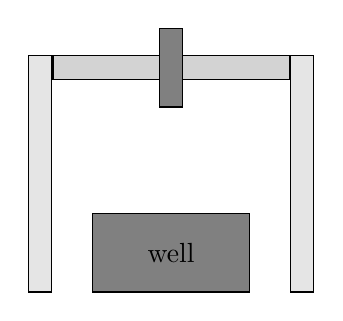
\begin{tikzpicture}
  \node[draw, fill=LightGrey, minimum height=3mm, minimum width=3cm](shaft){};
  \node at (shaft.north west)[anchor=north east, draw, fill=gray!20, minimum height=3cm, minimum width=3mm](lcol){};
  \node at (shaft.north east)[anchor=north west, draw, fill=gray!20, minimum height=3cm, minimum width=3mm](rcol){};
  \node at (lcol.south east) [anchor=south west, xshift=5mm, draw, fill=Grey, minimum width=2cm, minimum height=1cm]{well};
  \node at (shaft.center) [fill=Grey, draw, minimum width=3mm, minimum height=1cm](pulley){};
\end{tikzpicture}
\end{frame}

\begin{frame}[label={sec:org2f965e9}]{Solution}
Required power = (100 N)(0.5 m/s) = 50 W

So the given motor works, assuming 100\% efficiency

Assuming constant speed operation, required torque = 100(0.2) = 20 N-m = Torque on shaft

Force on shaft = Rope tension = 100 N
\end{frame}

\begin{frame}[label={sec:orgc5c15fe}]{Solution}
Shaft:

\begin{align*}
  \sigma_{a} &= \frac{100(1)r}{4(\pi/4)r^{4}} = \frac{31.8}{r^3} \\
  \sigma_{m} &= 0 \\
  \tau_{a} &= 0 \\
  \tau_{m} &= \frac{20(r)}{(\pi/2)r^{4}} = \frac{12.7}{r^3}
\end{align*}
\end{frame}

\begin{frame}[label={sec:orgb471e2f}]{Solution}
Calculating equivalent amplitude and mean stresses
\begin{align*}
  \sigma_{ae} &= \sqrt{\sigma_{a}^{2} + 3 \tau_{a}^{2}} = \frac{31.8}{r^{3}} \\
  \sigma_{me} &= \sqrt{\sigma_{m}^{2} + 3 \tau_{m}^{2}} = \sqrt{3}\frac{12.7}{r^{3}} = \frac{22}{r^3}
\end{align*}

Using Soderberg criteria,
\begin{align*}
  \frac{1}{N_{s}} &= \frac{\sigma_{ae}}{S_{e}} + \frac{\sigma_{me}}{S_{y}} \\
  \frac{1}{2} &= \frac{31.8}{r^{3}(0.5)(400 \times 10^{6})} + \frac{22}{r^{3}(300 \times 10^{6})} \\
  r^{3} &= 4.65 \times 10^{-7} \\
  r &= 7.75 \times 10^{-3} \text{ m}
\end{align*}
\end{frame}

\begin{frame}[label={sec:org42d61bc}]{Solution}
Disc Clutch: \(\mu = 0.1\)

A clutch -- use wet lining.

\begin{center}
\includegraphics[height=0.4\textheight]{./pictures/dry-materials.png}
\end{center}
\end{frame}

\begin{frame}[label={sec:orgc532e64}]{Solution}
Pick woven material so that \(p_{\max}\) = 500 kPa

Take \(r_i = 0.6 r_o\), number of disc \(N = 1\), safety factor \(N_s\) = 2.

\begin{align*}
  T_{design} &= N_s T = \mu \pi p_{\max} r_i \left( r_o^2 - r_i^2 \right) \\
  2(20) &= (0.1) \pi (500 \times 10^3) (0.6 r_o) \left( r_o^2 - (0.6r_o)^2 \right) \\
  r_o &= 0.087 \text{ m}
\end{align*}
\end{frame}

\begin{frame}[label={sec:orge313e0e}]{Solution}
Bearings:

Radial force = 100 N

Axial force is calculated from actuating force on clutch

\begin{align*}
    F &= p_{\max} \pi \left( r_o^2 - r_i^2 \right) \\
        &= 7609 \text{ N}
\end{align*}

Use angular contact since large axial load.

\begin{align*}
  \frac{F_a}{F_r} &= 47.8 \\
  F_e &= 0.911F_a \\
                  &= 6932 \text{ N}
\end{align*}
\end{frame}

\begin{frame}[label={sec:org7e65041}]{Solution}
\begin{center}
\includegraphics[width=0.7\textwidth]{./pictures/bearing-rated-capacity.png}
\end{center}

No other specifications, so assume reliability factor = 1, required life = \(9 \times 10^7\)

Application bearings are Xlt(55 mm), lt(35 mm), med(25 mm) = L11, 207, 305

All bearings have larger bore diameter than those required for the shaft. = Any of them works
\end{frame}


\begin{frame}[label={sec:org37c901c}]{Solution}
Recalculate shaft to account for axial load

\begin{align*}
  \sigma_{a} &= \frac{100(1)r}{4(\pi/4)r^{4}} = \frac{31.8}{r^3} \\
  \sigma_{m} &= \frac{7609}{\pi r^2} = \frac{2422}{r^2} \\
  \tau_{a} &= 0 \\
  \tau_{m} &= \frac{20(r)}{(\pi/2)r^{4}} = \frac{12.7}{r^3}
\end{align*}
\end{frame}

\begin{frame}[label={sec:org20cc5e5}]{Solution}
\begin{align*}
  \sigma_{ae} &= \sqrt{\sigma_{a}^{2} + 3 \tau_{a}^{2}} = \frac{31.8}{r^{3}} \\
  \sigma_{me} &= \sqrt{\sigma_{m}^{2} + 3 \tau_{m}^{2}} = \sqrt{\left(\frac{2422}{r^2}\right)^2 + 3 \left(\frac{12.7}{r^{3}} \right)^2}
\end{align*}

Using Soderberg criteria,

\begin{align*}
  \frac{1}{N_{s}} &= \frac{\sigma_{ae}}{S_{e}} + \frac{\sigma_{me}}{S_{y}} \\
  \frac{1}{2} &= \frac{31.8}{r^{3}(0.5)(400 \times 10^{6})} + \frac{\sqrt{\left(\frac{2422}{r^2}\right)^2 + 3 \left(\frac{12.7}{r^{3}} \right)^2}}{(300 \times 10^{6})} \\
\end{align*}

This must be solved analytically: \(r\) = 0.008 m = 8.0 mm
\end{frame}

\begin{frame}[label={sec:orgfc8365b}]{Solution}
Check buckling,

\begin{align*}
  N_s &= \frac{P_{cr}}{F_{comp}} \\
  P_{cr} &= 2(4782) = \frac{\pi^2 E I}{L_e^2} \\
  I &= \frac{\pi r^4}{4} = \frac{2(4782)(1)^2}{\pi^2(210 \times 10^9)} \\
  r &= 8.76 \times 10^{-3} \text{ m}
\end{align*}
\end{frame}

\begin{frame}[label={sec:org9b6f980}]{Summary}
\begin{itemize}
\item Many more variations of possible answers
\item Different choices of steel, linings, factors will lead to different answers
\end{itemize}
\end{frame}
\end{document}